\documentclass[11pt]{article}
\usepackage[margin=1in]{geometry}
\usepackage{enumerate}
\usepackage{framed}
\usepackage{multirow}
\usepackage{multicol}
\usepackage{bm}
\usepackage{amssymb}
\usepackage{amsmath}
\usepackage{amsthm}
\usepackage{multicol}
\usepackage{graphicx}
\usepackage{float}
\setlength{\columnsep}{1in}
\begin{document}

\newcommand{\Name}[1]{\noindent \textbf{Name:} #1 \\}
\newcommand{\pderiv}[2]{\frac{\partial #1}{\partial #2}}
\newcommand{\psderiv}[3]{\frac{\partial^2 #1}{\partial #2 \partial #3}}

\begin{center}
	\bf
	Machine Learning \\
	Computer Science 158 \\
	Spring 2017 \\
	\rm
	Project 7\\
\end{center}
\noindent \textbf{Name: Varsha Kishore and Savannah Baron} \\

\begin{enumerate}[1]
\item PCA and Image Reconstruction
\begin{enumerate}[(a)]
\item The average face seems to face on common features like eyes, nose and mouth that are in every picture in the data set. 
\item In the first 12 principle components, we can see different images representing different aspects of faces that might offer the most variance. For instance, in the first three, there is a lot of emphasis on color and face shape, where as the 8th we see features, and in the last two we see what seem to be faces ordered in different directions.  The principle components seek to explain the highest variance dimensions of the data. Thus, by emphasizing features such as face shape, eyes/mouth/nose and face angle, the principle components here represent important elements of faces.
\item Some people seem to be represented more clearly with lower $l$'s. For some of the other faces we need $l$ to be $100$ or higher for the face to become clear. 
\end{enumerate}
\item $K$-Means and $K$-Medoids
\begin{enumerate}[(a)]
\item This is a bad idea because the quantity $J$ will be minimized when the number of clusters
is $n$, and each cluster centroid corresponds to a data point in the training set. In other words, if we
also minimize with respect to $k$, we will massively overfit the data. 
\item Code complete!
\item Code complete!
\item Code complete!
\item Code complete!
\end{enumerate}
\item Clustering Faces
\begin{enumerate}[(a)]
\item \begin{tabular}{| c | c | c | c |}
  \hline		
   & Average & Min & Max \\
  \hline
  k-means & 0.616875 & 0.55 & 0.775 \\
  k-medoids & 0.63125 & 0.575 & 0.725   \\
  \hline
\end{tabular}\\ \\
TODO
\item 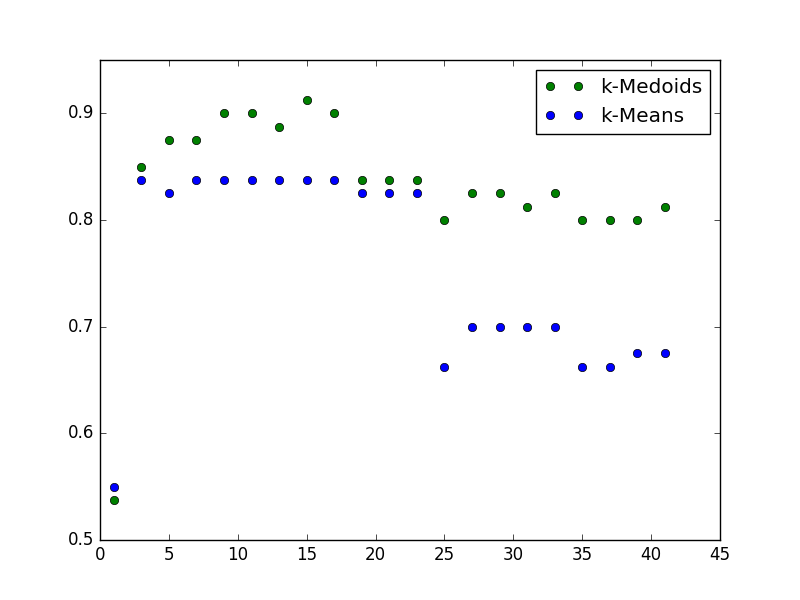
\includegraphics[scale=0.7]{figure_1}
\item TODO
\end{enumerate}
\end{enumerate}


\end{document}
